%% 
%% Copyright 2007-2024 Elsevier Ltd
%% 
%% This file is part of the 'Elsarticle Bundle'.
%% ---------------------------------------------
%% 
%% It may be distributed under the conditions of the LaTeX Project Public
%% License, either version 1.3 of this license or (at your option) any
%% later version. The latest version of this license is in
%%  http://www.latex-project.org/lppl.txt
%% and version 1.3 or later is part of all distributions of LaTeX
%% version 1999/12/01 or later.
%% 
%% The list of all files belonging to the 'Elsarticle Bundle' is
%% given in the file `manifest.txt'.
%% 
%% Template article for Elsevier's document class `elsarticle'
%% with numbered style bibliographic references
%% SP 2008/03/01
%% $Id: elsarticle-template-num.tex 249 2024-04-06 10:51:24Z rishi $
%%
\documentclass[preprint,12pt]{elsarticle}

%% Use the option review to obtain double line spacing
%% \documentclass[authoryear,preprint,review,12pt]{elsarticle}

%% Use the options 1p,twocolumn; 3p; 3p,twocolumn; 5p; or 5p,twocolumn
%% for a journal layout:
%% \documentclass[final,1p,times]{elsarticle}
%% \documentclass[final,1p,times,twocolumn]{elsarticle}
%% \documentclass[final,3p,times]{elsarticle}
%% \documentclass[final,3p,times,twocolumn]{elsarticle}
%% \documentclass[final,5p,times]{elsarticle}
%% \documentclass[final,5p,times,twocolumn]{elsarticle}

%% For including figures, graphicx.sty has been loaded in
%% elsarticle.cls. If you prefer to use the old commands
%% please give \usepackage{epsfig}

%% The amssymb package provides various useful mathematical symbols
\usepackage{amssymb}
%% The amsmath package provides various useful equation environments.
\usepackage{amsmath}
%% The amsthm package provides extended theorem environments
%% \usepackage{amsthm}
\usepackage{float}
%% The lineno packages adds line numbers. Start line numbering with
%% \begin{linenumbers}, end it with \end{linenumbers}. Or switch it on
%% for the whole article with \linenumbers.
%% \usepackage{lineno}

%% Added by author
\usepackage{hyperref}
\hypersetup{
  pdftitle={Measuring NASA Science Plan Alignment with Scientific Consensus: A Case Study in Space Science},
  pdfauthor={Richard H. Witt, Anamaria Berea},
  colorlinks=true,   % true: colored links instead of boxes
  linkcolor=blue,   % color of internal links
  urlcolor=blue,    % color of external links/URLs
  citecolor=blue,   % color of citation links
  filecolor=blue,   % color of file links
  pdfborderstyle={/S/U/W 1} % underline links instead of boxes
}
\usepackage[table]{xcolor}    
\usepackage{booktabs}
\usepackage{colortbl}   
\definecolor{A6GreyBlue}{HTML}{5686AA}
\definecolor{A6GreyGrey}{HTML}{7d93a0}
\definecolor{A6LightGrey}{HTML}{E5E9EC}

\journal{Space Policy Journal}

\begin{document}

\begin{frontmatter}

%% Title, authors and addresses

%% use the tnoteref command within \title for footnotes;
%% use the tnotetext command for theassociated footnote;
%% use the fnref command within \author or \affiliation for footnotes;
%% use the fntext command for theassociated footnote;
%% use the corref command within \author for corresponding author footnotes;
%% use the cortext command for theassociated footnote;
%% use the ead command for the email address,
%% and the form \ead[url] for the home page:
%% \title{Title\tnoteref{label1}}
%% \tnotetext[label1]{}
%% \author{Name\corref{cor1}\fnref{label2}}
%% \ead{email address}
%% \ead[url]{home page}
%% \fntext[label2]{}
%% \cortext[cor1]{}
%% \affiliation{organization={},
%%       addressline={},
%%       city={},
%%       postcode={},
%%       state={},
%%       country={}}
%% \fntext[label3]{}

\title{Measuring NASA Science Plan Alignment with Scientific Consensus: A Case Study in Space Science}

%% Alternative title 1: if I add budget analysis
%%\title{Science, Policy, and Money: How Science gets funded in the United States}

%% use optional labels to link authors explicitly to addresses:
%% \author[label1,label2]{}
%% \affiliation[label1]{organization={},
%%       addressline={},
%%       city={},
%%       postcode={},
%%       state={},
%%       country={}}
%%
%% \affiliation[label2]{organization={},
%%       addressline={},
%%       city={},
%%       postcode={},
%%       state={},
%%       country={}}

\author[1]{Richard Witt\corref{cor1}}
\ead{rwitt4@gmu.edu}

\author[2]{Anamaria Berea}
% \ead{aberea@gmu.edu}

\affiliation[1]{organization={Computational and Data Sciences, PhD Student,George Mason University},
      addressline={4400 University Drive}, 
      city={Fairfax},
      postcode={22030}, 
      state={Virginia},
      country={USA}}

\affiliation[2]{organization={Computational Social Sciences, Associate Professor, George Mason University},
      addressline={4400 University Drive}, 
      city={Fairfax},
      postcode={22030}, 
      state={Virginia},
      country={USA}}

\cortext[cor1]{Corresponding author}

%%%%%%%%%%%%%%%%%%%%%%%%%%%%%%%%%%%%%%%%%%%%%%%%%%%%%%%%%%%%%%%%%%%%%%%%%%%%%%%%%%%
% Abstract
%%%%%%%%%%%%%%%%%%%%%%%%%%%%%%%%%%%%%%%%%%%%%%%%%%%%%%%%%%%%%%%%%%%%%%%%%%%%%%%%%%%
\begin{abstract}
%% Text of abstract
The National Academies of Science Engineering and Medicine conducts Decadal Surveys which NASA uses to prioritize future endeavors. The article investigates how science plans at NASA align with scientific community consensus identified in the decadal surveys. Natural Language Processing was used to compare semantic similarity between decadal surveys and NASA science plans. A group of 4 decadal surveys from 2001 to 2007 was used to create a baseline. NASA science plan alignment was then measured against this baseline. Alignment between science plans with baseline decadal surveys is shown to decrease over time. This decreased alignment over time indicates a potential decreasing effect of earlier decadal surveys on later science plans as consensus shifts, new decadal surveys are created, and operational realities change. The article serves as an initial investigation of semantic similarity as a potential methodology of determining alignment across large and separate organizations. 

\end{abstract}

%%Graphical abstract
\begin{graphicalabstract}
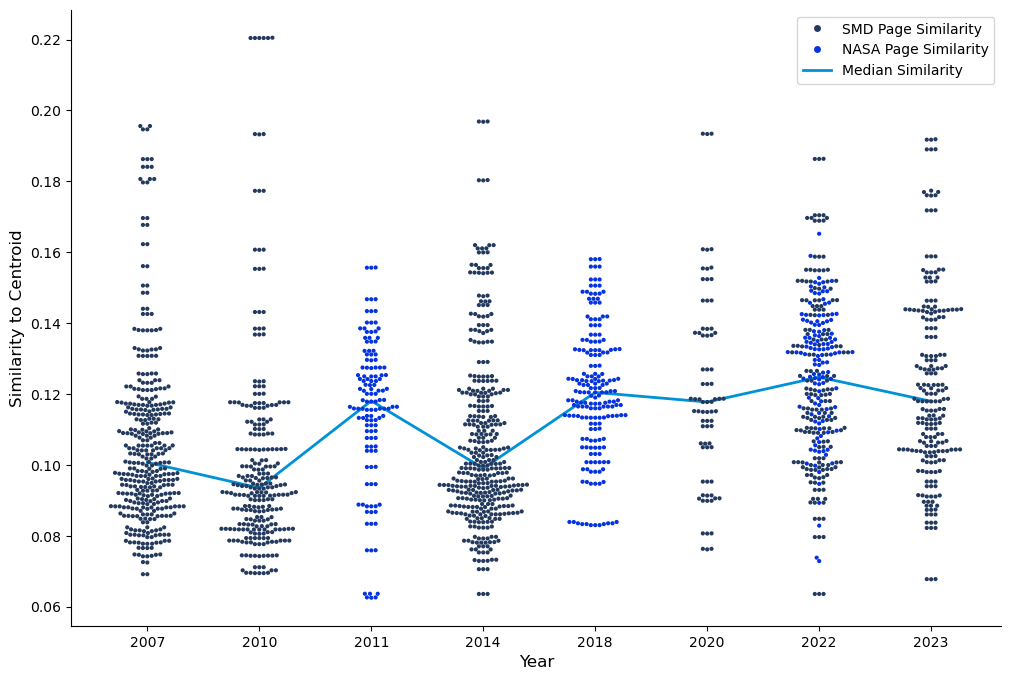
\includegraphics[width=0.9\textwidth]{fig_graphical_abstract.png}
\end{graphicalabstract}

%%Research highlights
\begin{highlights}
\item Investigation of NASA Space Science Plans alignment with decadal surveys
\item Natural language processing with context embeddings used for comparison
\item NASA Science plan alignment with decadal surveys decreased over time
\end{highlights}

%% Keywords
\begin{keyword}
%% keywords here, in the form: keyword \sep keyword
NASA science policy \sep decadal surveys \sep policy alignment \sep natural language processing \sep context embeddings \sep semantic similarity \sep science planning \sep space science

%% PACS codes here, in the form: \PACS code \sep code
\PACS 01.78.+p \sep 89.20.Dd \sep 01.75.+m \sep 89.70.Cf
% 01.78.+p (Science and government)
% 89.20.Dd (Space science policy and planning)
% 01.75.+m (Science and society)
% 89.70.Cf (Information and communication theory)

%% MSC codes here, in the form: \MSC code \sep code
\MSC 68T50 \sep 91B82 \sep 62P12 \sep 91F99
% 68T50 (Natural language processing)
% 91B82 (Statistical methods; economic indices and measures)
% 62P12 (Applications of statistics to environmental and related topics)
% 91F99 (Other social and behavioral sciences)
\end{keyword}

\end{frontmatter}

%% Add \usepackage{lineno} before \begin{document} and uncomment 
%% following line to enable line numbers
% \linenumbers

%% main text
%%

%%%%%%%%%%%%%%%%%%%%%%%%%%%%%%%%%%%%%%%%%%%%%%%%%%%%%%%%%%%%%%%%%%%%%%%%%%%%%%%%%%%
% Introduction and Literature Review
%%%%%%%%%%%%%%%%%%%%%%%%%%%%%%%%%%%%%%%%%%%%%%%%%%%%%%%%%%%%%%%%%%%%%%%%%%%%%%%%%%%
\section{Introduction and Literature Review}

% For review: This is abstract, not introduction. The Introduction outlines the problem and the structure of the paper.

NASA alignment with scientific community interests in science discovery is of major importance to the scientific community. Still, limited research has been conducted on this alignment with only two studies seeking to identify this relationship \cite{Trimble2011} \cite {pan2023seven_decadals}. Further, these studies focus solely on Astronomy and Astrophysics. We aim to observe project alignment across all NASA Science Mission Directorates using natural language processing techniques. 

Creating a strategic plan for United States science discovery is a multi-agency, multi-year planning process. Two key corpora result from this planning process. The first corpus is U.S. National Academies of Science, Engineering, and Medicine (Academies) created decadal surveys. The second corpus is composed of NASA strategic plans, and NASA Science Mission Directorate science plans. In this paper we reefer to strategic and science plans collectively as NASA plans. NASA plans are used to define NASA project priorities while Decadal Surveys are used to identify scientific community interests.

\subsection{Decadal Surveys}

%For Review: You need to explain better how the Decadal surveys work.

Decadal surveys are a strategic guide for the planning and execution of United States investments in Science and Technology\cite{Academies2015_lessons}. The purpose of decadal surveys is to reach consensus on science priorities for the next decade while aligning with the executive branch initiatives and adhering to fiscal budget constraints. The Space Studies Board at the Academies reviewed lessons learned and best practices for prior decadal surveys in 2015. The bulk of this section relies on this work except where otherwise cited \cite{Academies2015_lessons}.

Decadal surveys are important to the entire scientific community. Survey chairs and committee members are accomplished scientist and engineers who are active leaders in their field from top institutions and universities in the United States. A review of decadal survey committee and panel members reads like a who's who of science and engineering. NASA and National Science Foundation (NSF) officials refer to the decadal survey recommendations as a blueprint or guidebook and individual research scientists refer to the surveys as a "sword and shield". A sword for wining approval and shield against cancellation of federally funded programs. Independent studies of surveys in 2011 \cite{Trimble2011} and 2023 \cite{pan2023seven_decadals} both found that around 60\% of projects identified in decadal surveys are funded within 15 years of survey publication. 

Stakeholders in the decadal surveys include many U.S. government agencies, departments, and foundations. NASA's Science Mission Directorate (SMD) is a common sponsor of the decadal surveys along with the NSF. Additional science community stakeholders in the decadal surveys include DOE, NOAA, and USGS. Congress, the Office fo Management and Budget, and other executive branch agencies use decadal surveys to evaluate budgetary plans.

This multi-agency, multi-stakeholder, arrangement as well as the considerable workload, high standards, and complexity of the task causes the process of conducting decadal surveys to be necessarily long and complex. The process starts with the Academies creating a statement of task for the committee to respond to. The Academies' Space Studies Board works with other standing committees at the Academies to select a survey chair and committee of around 20 members. The survey committee, with help from the Academies staff, organize panels and working groups by science themes, observational techniques, facilities, or subject. This freedom of organization allows for the culture of the scientific field and preference of the survey organizers to mold the committee. The surveys gather broad community input through public meetings, "white papers", and direct presentations. The panels then create a ranked program of missions and activities based on science and observational capabilities specific to the panels area of responsibility. Panel priorities are then ranked across the field by the survey committee. 

Independent reviews ensure scientific and fiscal rigor. Once panels and committees have completed their work independent cost and risk evaluation is conducted for larger space missions and ground based facilities as mandated by the U.S. Congress \cite{congress2008NASA}. The committee's report also undergoes an independent review to validate conclusions are supported and documented. The final report takes around 2 years to complete and provide a consensus vision of for its respective field.

Followup on decadal surveys requires multi-agency involvement. Once the survey report is published the committee is disbanded. Post report stewardship is conducted by standing committees at the Space Studies Board through periodic reviews which offer guidance to the agencies on decadal programs. The NASA Advisory Council's Science subcommittees at the Academies follow NASA's progress. A congressionally directed midterm review of decadal surveys focus on agency progress to compare activities with survey science goals is also conducted \cite{congress2005nasa}. The National Science Foundation receives input from the scientific community through proposals to it's various programs. The Department of Energy evaluates progress through extensive internal processes for energy related components of the surveys while independent committees such as the Astrophysics Advisory Committee, provide advisory services on multi-agency projects.

Decadal surveys serve as a national science strategy and are intended to inform science strategy at NASA and other federal agencies. 

\subsection{NASA Science Strategy}
%For Review: You need to explain more what the NASA strategy is and how it is created.
NASA relies heavily on decadal surveys to inform its science strategy. NASA's 2025 Presidents Budget Request states "SMD uses the recommendations of the National Academies' decadal surveys as important inputs in planning and prioritizing the future of its science programs." The same budget references decadal surveys 87 times demonstrating NASA's focus on the surveys to define science strategy \cite{NASA2025budget}. 

The decadal surveys are not the only input to NASA science strategy. The Office of the Chief Scientist (OCS) represents all of the scientific endeavors in the agency, ensuring they are aligned with and fulfill the administration's science objectives \cite{nasa_partnerships_2024}. International scientific consensus is also important since two-thirds of SMD missions involve international partnerships \cite{nasa_smd_hearing_2024}. 
 
Science strategy is further refined by operational realities. The SMD Large Mission Study (LMS) Report lays out the most current Simplified Project Lifecycle available. This report identifies 7 Project Life-Cycle Phases. 3 of which occur prior to implementation and are therefore germane to the the project prioritization process. These 3 phases are Phase Pre-A: Concept Studies, Phase A: Concept and Technology Development, and Phase B: Preliminary Design and Technology Completion. In this process decadal survey recommendations are turned into decisions on mission architectures, preliminary requirements and budget estimates. In the Pre-Phase-A period missions are not yet projects and focus is on quantifying science vs cost, exploiting the range of solutions while maintaining dialog with Academy committees to ensure the intent of the decadal survey is honored. Once Key Decision Point-A passed the concept is identified as executable and continues through the rest of the Concept Maturity Model to eventually become a project once Phase B is completed. \cite{NASA2020_LMS_study} \cite{wessen2013ConceptMaturity}.

The science strategy that results from this refinement process is defined in the NASA plans that are created. Since a large portion of the plan is natural language text additional processing is needed to extract information which can be measured using numerical methods. This information extraction is the process of creating word embeddings.

\subsection{Word and Context Embeddings}
Word embeddings are numerical interpretations of words that capture syntactic and semantic meaning for individual words \cite{mikolov2013_reps_of_words}, sentences \cite{reimers2019sentencebertsentenceembeddingsusing}, and documents \cite{wu_2018_doc_embeds}. These numerical interpretations, or word vectors, can be used to understand textual relationships mathematically. In 2013 Word2Vec extended \cite{mikolov2013_reps_of_words} and formalized \cite{mikolov2013_efficient_word_est} prior work by Bengio et al. \cite{bengio_2003_neural_prob_lang}. 

While early word embeddings were limited to a single global representation for each word the ELMo model \cite{peters2018deepcontextualizedwordrepresentations} used context-dependent inputs to capture meaning across diverse contexts, enabling the model to interpret words with polysemy thus beginning the era of Context Embedding models. BERT \cite{devlin2019bert_pretraining} added bidirectional encoding, GPT \cite{radford2018improving_GPT} added auto-regression prediction and BART \cite{lewis2019bart} combined these two innovations to increase performance on text generation tasks. Embedding models are used as an unsupervised stage prior to the supervised fine tuning stage for transformer based large language models since their inception \cite{vaswani2023attentionneed} and in current state of the art open source models \cite{grattafiori2024_llama3_herdmodels}.

Our research relies on OpenAI's \texttt{text-embedding-ada-002} model due to its favorable performance in document level search \cite{Aperdannier2024_embedding_search}. The model was released on December 15, 2022 \cite{openai2023ada_embeddings} as closed source. However, on January 24, 2022 OpenAI published Text and Code Embeddings by Contrastive Pre-Training \cite{neelakantan2022openAi_embeddings} indicating that \texttt{text-embedding-ada-002} is likely an evolution of this prior work using a contrastive objective on paired samples with relatedness evaluated using cosine similarity. 

\subsection{Outline}
The remainder of this paper is structured as follows: Section~\ref{meth} describes the methodology and rationale used to compare project priorities at NASA with scientific consensus using context embeddings. Section~\ref{data} details the source documentation used in the analysis. Section~\ref{anal_results} provides the analysis and results from the documentation comparison. Finally Section~\ref{discussion} discusses the results and describes potential paths for future work. 

%%%%%%%%%%%%%%%%%%%%%%%%%%%%%%%%%%%%%%%%%%%%%%%%%%%%%%%%%%%%%%%%%%%%%%%%%%%%%%%%%%%
% Methodology and rationale 
%%%%%%%%%%%%%%%%%%%%%%%%%%%%%%%%%%%%%%%%%%%%%%%%%%%%%%%%%%%%%%%%%%%%%%%%%%%%%%%%%%%
\section{Methodology and rationale}
\label{meth}
This analysis followed a methodology adapted from the CRoss Industry Standard Process for Data Mining (CRISP-DM)\cite{wirth2000crisp}. The methodology consists of idempotent process steps of Ingest, Prepare, Pre-process, Model, and Validate. This outline is shown in Figure~\ref{fig_DS_Process}.

\begin{figure}[H]
\centering
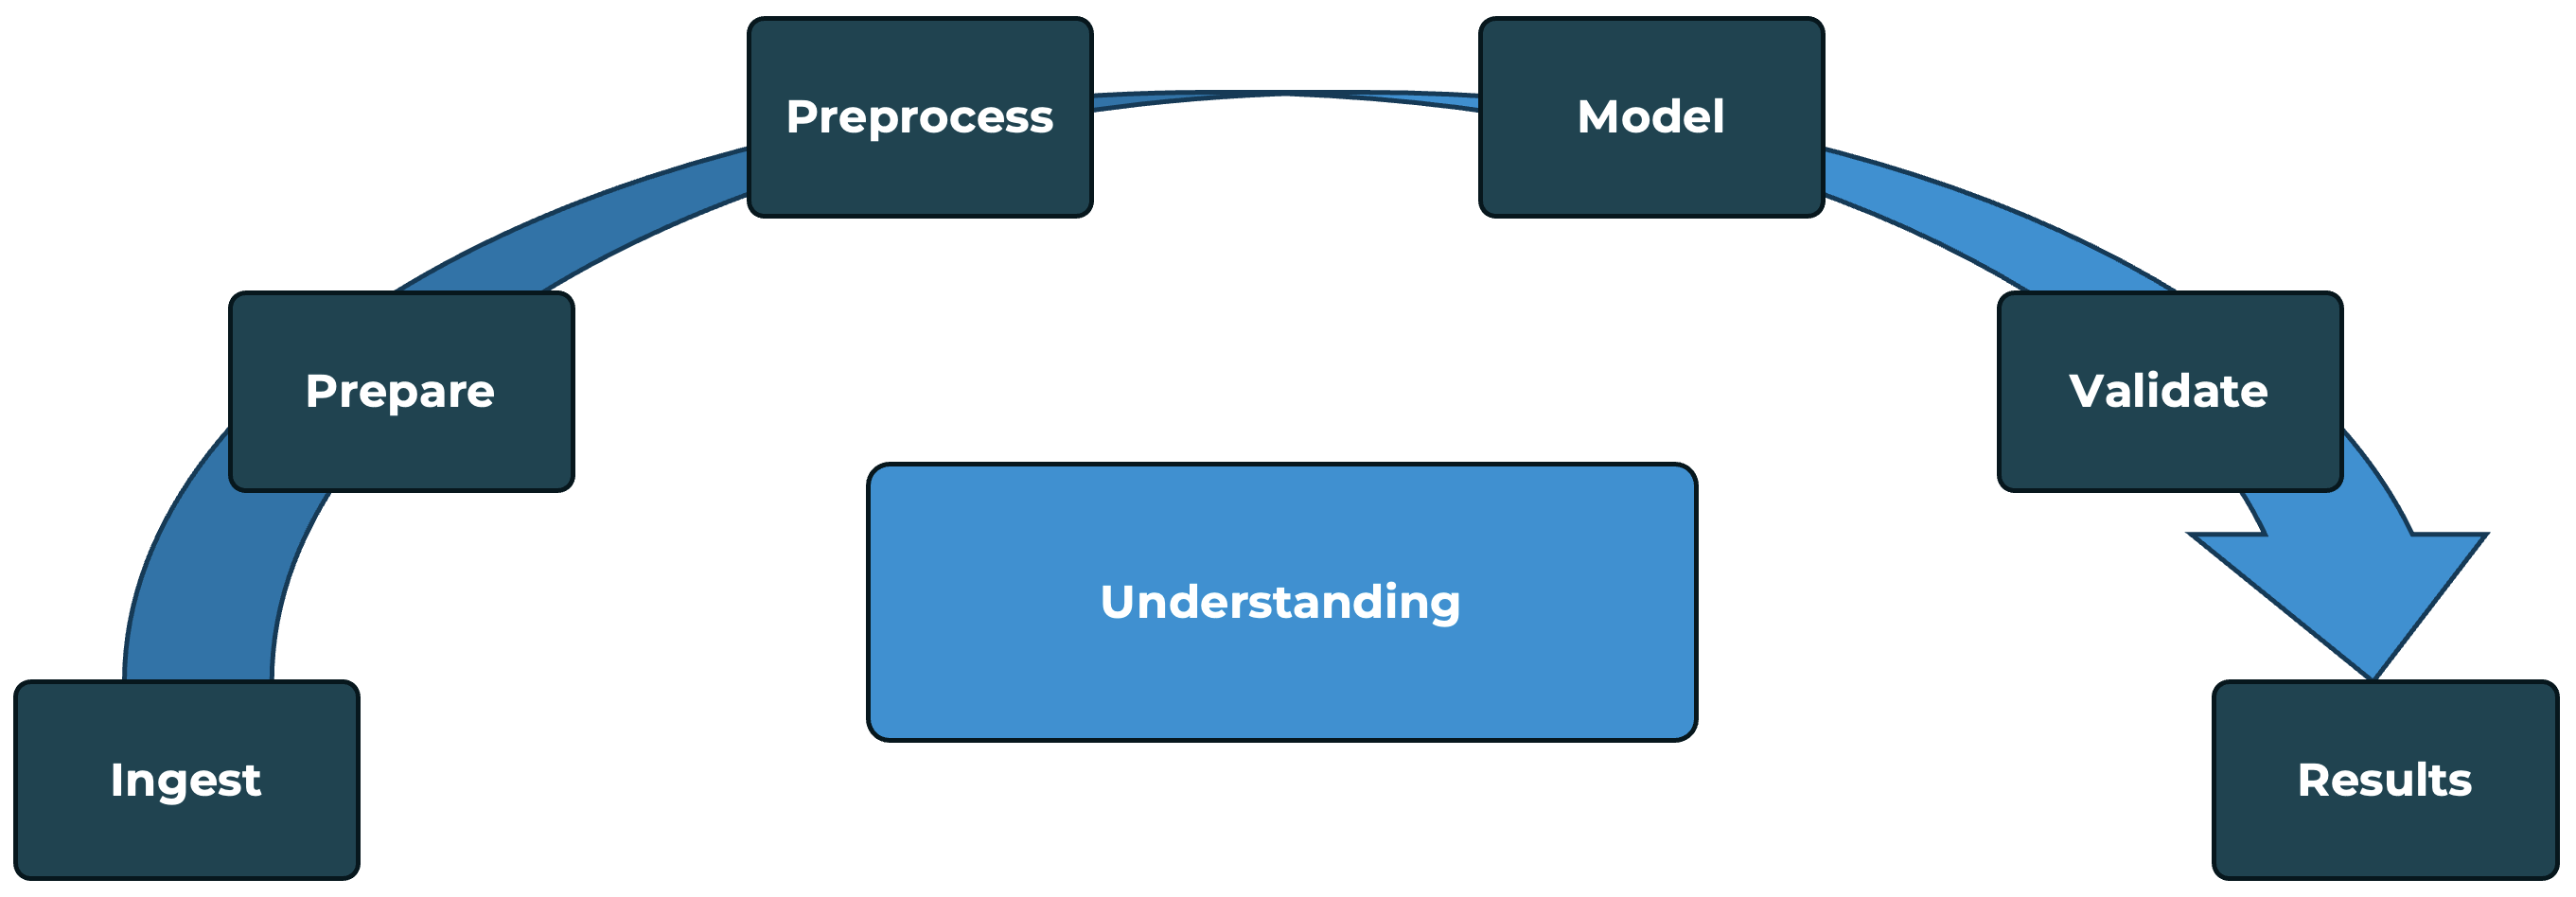
\includegraphics[width=0.9\textwidth]{fig_DS_Process.png}.
\caption{Core Data Science Process}\label{fig_DS_Process}
\end{figure}

\subsection{Ingesting Source Data}
Data ingestion was a manual process using file names to embed metadata into the the files. This metadata was then used programmatically in follow on processes. Metadata consisting of publication year, document category, and publication type were all encoded into the file names to ensure accurate processing. For information on the specific data used see the Section~\ref{data} Data.

Once data is ingested the next step is to prepare the data.

\subsection{Preparing the Text}
The first step in preparation is to extract the text from the pdf files. We completed this step with \texttt{PDFminer} which is a common PDF parser and analyzer\cite{pdfminer}. \texttt{PDFminer} extracted raw page text which is then cleaned with Python's \texttt{re} module which provides support for regular expressions. Regular expressions were used to remove patterns in text such as special characters used in PDF formatting, page numbers, and blank pages. Document metadata, such as year of publication, was then extracted from the file names and stored as metadata with text from each page resulting in a total corpus size of just over 800 pages of NASA science plans and decadal surveys. Each page of clean text with metadata was then stored for further preprocessing with contextual embeddings. 

Now that the data is prepared we can preprocess it for our specific analysis.

\subsection{Preprocessing with Contextual Embeddings}

Once the text is prepared each individual page is turned into a contextual embedding vector with 1536 dimensions using the \texttt{text-embedding-ada-002} model. High dimensional embeddings were chosen to leverage prior studies on document level search \cite{Aperdannier2024_embedding_search} and because we speculate that higher dimensionality may better represent the context, semantics, and syntactic meaning in a large chunk of text such as a page of a PDF document. 

After preprocessing the data is ready to be modeled. 

\subsection{Modeling with Contextual Comparison}
All contextually embedded pages for each individual corpus are then concatenated into a single index where all pages from all documents in the corpus are included in a single index. In the same way a Bag of Words model is a simple text representation that disregards word order and only accounts for how many times a word appears, this model could be viewed as a Bag of Pages model that disregards page order and only accounts for the similarity of each page to other pages in the corpus. Page order is disregarded and only similarity of each page to the rest of the pages in the corpus is modeled. 

In order to investigate the relationship between scientific consensus and NASA plans a hierarchical approach is used. Although NASA is not a subordinate of the NSF, NASA science plans should inherit information from decadal surveys. This creates informational hierarchy where information from the parent decadal survey corpus flows to the child NASA science plan corpus. 

The hierarchical relationship is modeled by creating a baseline of parent corpus documents which in this case is the decadal surveys. This baseline is computed by calculating a simple mean of page vectors constituting the parent corpus.  

Figure~\ref{fig_simple_context_dist} is a simplified representation of the contextual distance model used. $X_{1}$ and $X_{2}$ each represent a dimension used to compare the documents thus simplifying the high dimensionality space of 1532 dimensions into just two dimensions in order to visualize the concept.

\begin{figure}[H]
\centering
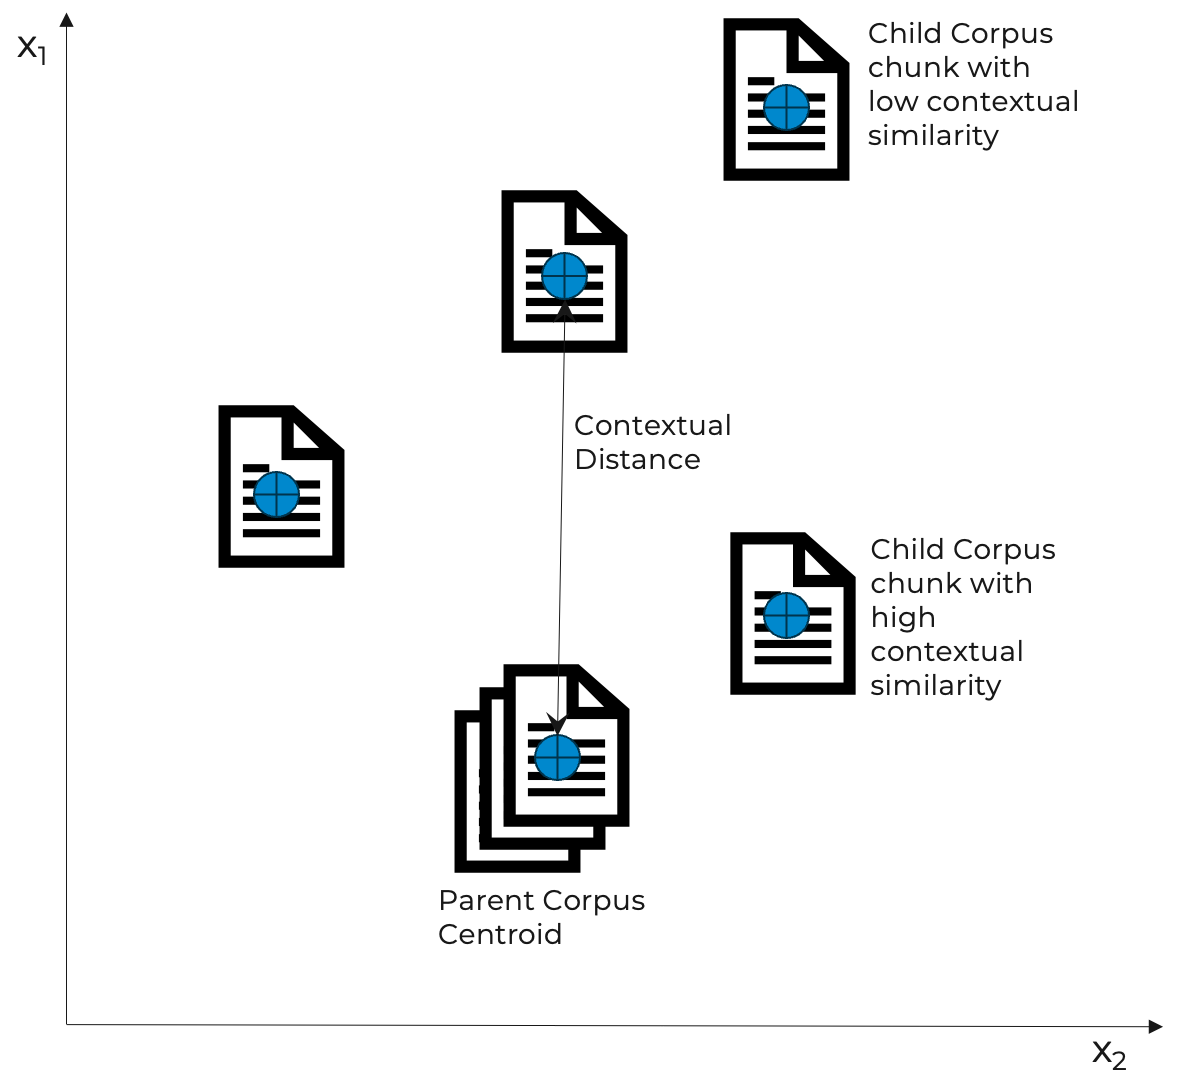
\includegraphics[width=0.7
\textwidth]{fig_simple_context_dist.png}
\caption{Simplified Contextual Distance Model}\label{fig_simple_context_dist}
\end{figure}

The distance of each page in the NASA plan is calculated from the decadal survey centroid. Cosine similarity was chosen to calculate the distance between documents due to the use of cosine similarity in the training of the original embeddings model. 

Selection of data for the model required some compromise which is explained in the next section. 

%%%%%%%%%%%%%%%%%%%%%%%%%%%%%%%%%%%%%%%%%%%%%%%%%%%%%%%%%%%%%%%%%%%%%%%%%%%%%%%%%%%
% Data
%%%%%%%%%%%%%%%%%%%%%%%%%%%%%%%%%%%%%%%%%%%%%%%%%%%%%%%%%%%%%%%%%%%%%%%%%%%%%%%%%%%
\section{Data}
\label{data}
\subsection{Decadal Surveys}
The National Research Council (NRC) of the Academies has conducted decadal surveys at approximately a 10 year cadence since 1964. Decadal surveys typically require 2 years to complete each survey \cite{Academies2015_lessons}. Until 2003 decadal surveys were focused on Astronomy and Astrophysics. However since then, Decadal surveys are listed into the following 5 categories: Astrophysics, Planetary, Heliophysics, Earth, and a final category of Biological and Physical.

The purpose of decadal surveys is to reach consensus on science priorities for the next decade while aligning with the executive branch initiatives and adhering to fiscal budget constraints. Science community stakeholders in the decadal surveys include NASA, NSF, DOE, NOAA, and USGS. Congress, the Office fo Management and Budget, and other executive branch agencies use decadal surveys to evaluate budgetary plans. Given the magnitude of impact of the studies, survey committees consist of experienced, active, and accomplished leaders in their respective fields \cite{Academies2015_lessons}.

Decadal surveys for this report were sourced directly from the National Academies Press website \cite{Academies_decadal}. NASA also lists the most recent Decadal Surveys on it's Science Mission Directorate website \cite{NASA_decadal}.

The distance of science plan pages is measured from the centroid of the decadal survey corpus. This was necessary because any single decadal survey covers only one of the NASA Science Mission Directorates while NASA Science Plans cover all 5 Science Mission Directorates. The centroid (median) of the 2001-2007 decadal surveys was chosen as those surveys cover 4 of the 5 SMDs. This eliminates Biological and Physical Sciences from the reference centroid because the first decadal survey for this SMD was not released until 2011. Including this survey would cause 3 of the 9 NASA science plans to occur after the last document in the decadal survey corpus thereby causing temporal leakage. 

\subsection{Science Strategy}
NASA Science plans define NASA Science strategy and cross all 5 decadal survey categories to provide guidance for each division of the SMD. 

NASA Science plans have two distinct sources. Three of the plans in the corpus are created as NASA Strategic Plans, signed by the NASA Administrator, and seven are Science Mission Directorate (SMD) Science Plans, signed by the Associate Administrator of the Science Mission Directorate\cite{SMD_2007} \cite{SMD_2010} \cite{NSP_2011} \cite{SMD_2014} \cite{NSP_2018} \cite{SMD_2020} \cite{NSP_2022} \cite{SMD_2022} \cite{SMD_2023} \cite{SMD_2025}.

 NASA Science Mission Directorate has a web page devoted to science strategy containing SMD Science Plans, NASA Strategic Plans, and accompanying documentation for most years beginning in 2007 \cite{NASA_sci_strat}. 

 The divisions of the SMD closely align to the decadal surveys and consist of 6 divisions reporting to the Deputy Associate Administrator \cite{NASA_SMD}. Four of the divisions are represented in Table~\ref{tab:decadals_used}. Joint Agency Satellite Division and Biological and Sciences Division are not mapped to the decadal surveys because Joint Agency Satellite has no corresponding decadal surveys and Biological and Physical Sciences first survey occurs after the first available science plan and was removed to avoid temporal leakage from science plans affecting decadal surveys.  

\subsection{Matching Surveys with Strategy to measure Context Similarity}
Four Decadal Surveys published between 2001 and 2007 were chosen to to determine if decadal survey effects are observable on NASA Science Plans using semantic similarity.  This reduction has two effects on our data sample. First it reduces the data to points in time prior to the first NASA Science Plan analyzed in the report. Second it creates a sample that represents a cross section matching the scope of NASA Science Plans. 

The sample of Decadal Surveys creates a baseline to observe semantic drift of NASA plans that happens after decadal surveys are published. Semantic drift is defined here as the rate of separation of one corpus of text from another over time. The surveys used in this analysis along with the year published and corresponding NASA SMD Division the survey relates to is shown in Table~\ref{tab:decadals_used}. For a complete table of surveys see \ref{app_decadal_surveys}.

\begin{table}[H]
\centering
\begin{tabular}{p{1.2cm} p{7.5cm} p{3.5cm}}
 \hline
 \rowcolor[gray]{0.95}
 \textbf{Year} & \textbf{Title} & \textbf{Corresponding SMD Division} \\ \hline
 2001 & Astronomy and Astrophysics for the New Millennium & Astrophysics \\
 \rowcolor[gray]{0.97}
 2003 & The Sun to the Earth—and Beyond: A Decadal Research Strategy in Solar and Space Physics & Heliophysics \\
 2003 & New Frontiers in the Solar System: An Integrated Exploration Strategy & Planetary  Science \\
 \rowcolor[gray]{0.97}
 2007 & Earth Science and Applications from Space: National Imperatives for the Next Decade and Beyond & Earth Science \\
\end{tabular}
\caption{Decadal Surveys Used in Analysis \cite{Academies_decadal, NASA_sci_strat}}\label{tab:decadals_used}
\end{table}
%%%%%%%%%%%%%%%%%%%%%%%%%%%%%%%%%%%%%%%%%%%%%%%%%%%%%%%%%%%%%%%%%%%%%%%%%%%%%%%%%%%
% results
%%%%%%%%%%%%%%%%%%%%%%%%%%%%%%%%%%%%%%%%%%%%%%%%%%%%%%%%%%%%%%%%%%%%%%%%%%%%%%%%%%%
\section{Analysis and Results} 
\label{anal_results}

The distance between decadal survey and science plans is measured using cosine similarity. The baseline of decadal surveys is assigned a distance value of 0. A perfectly aligned page would have a distance of 0 and lie directly on the axis. Individual pages of NASA plans are represented by points shown in Figure~\ref{fig2}. Finally the median similarity of the NASA plan pages is represented by the line plot. 

\begin{figure}[H]%% placement specifier
%% Use \includegraphics command to insert graphic files. Place graphics files in 
%% working directory.
\centering%% For centre alignment of image.
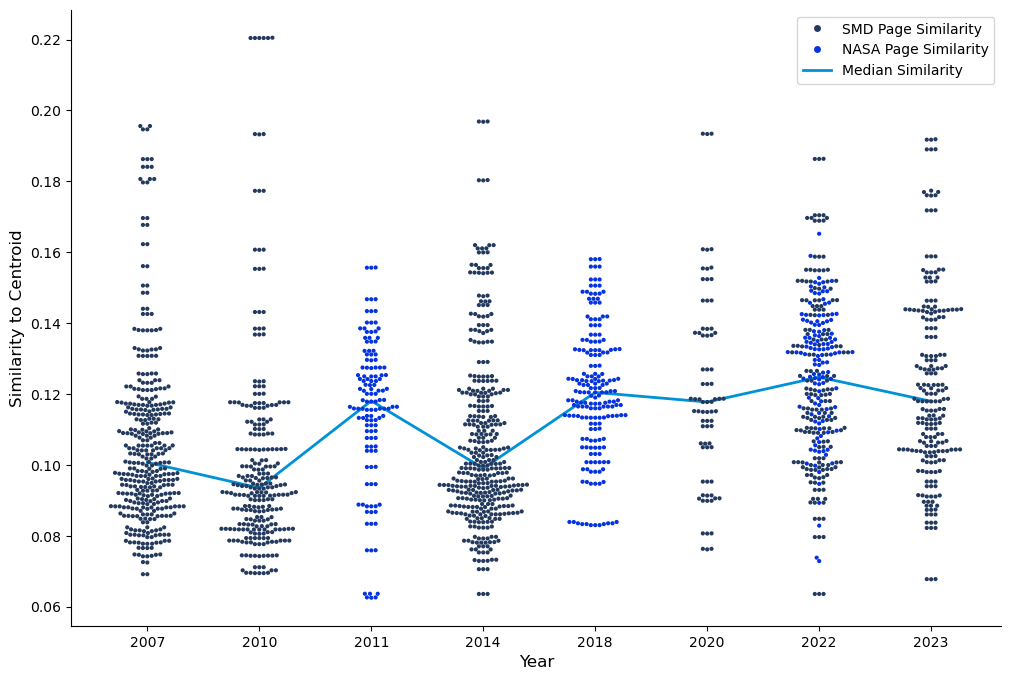
\includegraphics[width=0.9\textwidth]{fig_SP_to_DS_similarity.png}
%% Use \caption command for figure caption and label.
\caption{NASA Science Plan Similarity to Decadal Surveys}\label{fig2}
%% https://en.wikibooks.org/wiki/LaTeX/Importing_Graphics#Importing_external_graphics
\end{figure}

We can observe two patterns from Figure~\ref{fig2}. First the median similarity of the NASA plans in relation to decadal surveys is decreasing over time. Second there is a difference between NASA led plans and SMD led plans as shown by the different colors representing the pages in each corpus.  SMD led plan pages tend to be closer to the decadal survey centroid. 
%%%%%%%%%%%%%%%%%%%%%%%%%%%%%%%%%%%%%%%%%%%%%%%%%%%%%%%%%%%%%%%%%%%%%%%%%%%%%%%%%%%
% Discussion
%%%%%%%%%%%%%%%%%%%%%%%%%%%%%%%%%%%%%%%%%%%%%%%%%%%%%%%%%%%%%%%%%%%%%%%%%%%%%%%%%%%
\section{Discussion and Future Work}
\label{discussion}

The decreased alignment over time between NASA plans and decadal surveys likely has many causal factors. In addition to decadal surveys NASA must has many other competing influences in science plans. We can conjecture that the decreased alignment may be a result of changes in consensus as surveys are updated, changes in executive branch priorities, changes in congressional funding, or changes in operational realities. This introduces multiple vectors that are not accounted for in an analysis that focuses on decadal surveys and time. The limited amount of data due to the once a decade periodicity of survey publication limits the conclusions that can be drawn. 

The analogous results that are observable provide encouragement that measuring the change in semantic similarity may be a useful analysis methodology and provides several areas for further study. This particular study could be expanded by categorizing decadal surveys into the 5 SMD divisions and exploring a more fine grained analysis of each scientific community. As a general approach, cross corpus contextual similarity analysis may be useful in other other areas where cross organizational alignment is a concern.  The approach could be extended by comparing page level, or smaller pieces of text across corpora by means of clustering algorithms. Optimization of architecture could also be explored by optimizing for embeddings models and hyperparameters.   


%%%%%%%%%%%%%%%%%%%%%%%%%%%%%%%%%%%%%%%%%%%%%%%%%%%%%%%%%%%%%%%%%%%%%%%%%%%%%%%%%%%
% appendix
%%%%%%%%%%%%%%%%%%%%%%%%%%%%%%%%%%%%%%%%%%%%%%%%%%%%%%%%%%%%%%%%%%%%%%%%%%%%%%%%%%%
\newpage 
\appendix
\section{Complete List of Decadal Surveys}
\label{app_decadal_surveys}
A complete list of Decadal Surveys is given in Table \ref{tab:decadals_all}. The table also incudes a Lessons Learned and Best Practices report conducted as a review of decadal surveys conducted in 2015. For researchers interested in learning more about this is a great resource \cite{Academies2015_lessons}.

\begin{table}[H]
\centering
\begin{tabular}{p{1.2cm} p{8.5cm} p{2.9cm}}
 \hline
 \rowcolor[gray]{0.95}
 \textbf{Year} & \textbf{Title} & \textbf{Corresponding SMD Division} \\

 1964 & Ground-based Astronomy a Ten-Year Program & Astrophysics \\

 1973 & Astronomy and Astrophysics for the 1970s & Astrophysics \\

 1982 & Astronomy and Astrophysics for the 1980s & Astrophysics \\

 1991 & A Decade of Discovery in Astronomy and Astrophysics & Astrophysics \\

 2001 & Astronomy and Astrophysics for the New Millennium & Astrophysics \\

 2003 & The Sun to the Earth—and Beyond: A Decadal Research Strategy in Solar and Space Physics & Heliophysics \\

 2003 & New Frontiers in the Solar System: An Integrated Exploration Strategy & Planetary Science \\

 2007 & Earth Science and Applications from Space: National Imperatives for the Next Decade and Beyond & Earth Science \\

 2010 & New Worlds, New Horizons in Astronomy and Astrophysics & Astrophysics \\

 2011 & Recapturing a Future for Space Exploration: Life and Physical Sciences Research for a New Era (2011) & Biological and Physical Sciences \\

 2011 & Vision and Voyages for Planetary Science in the Decade 2013-2022 & Planetary Science \\

 2013 & Solar and Space Physics: A Science for Technological Society & Heliophysics \\

 2015* & The Space Science Decadal Surveys: Lessons Learned and Best Practices (2015) & N/A \\

 2018 & A Midterm Assessment of Implementation of the Decadal Survey on Life and Physical Sciences Research at NASA (2018) & Planetary Science \\

 2018 & Thriving on Our Changing Planet: A Decadal Strategy for Earth Observation from Space & Earth Science \\

 2023 & Pathways to Discovery in Astronomy and Astrophysics for the 2020s (2023) & Astrophysics \\

 2023 & Thriving in Space: Ensuring the Future of Biological and Physical Sciences Research: A Decadal Survey for 2023-2032 (2023) & Biological and Physical Sciences \\

 2023 & Origins, Worlds, and Life: A Decadal Strategy for Planetary Science and Astrobiology 2023-2032 (2023) & Planetary Science \\

\end{tabular}
\caption{NASA Science Mission Directorate Decadal Surveys}\label{tab:decadals_all}
\end{table}

\section{File Name Metadata}
\label{app_file_names}
This section details the file name convention used in this analysis and is provided to aid in future work. It is available at TODO: PUBLIC REPO. 

\begin{description}
 \item[Decadal file names:] Follow a \texttt{yyyy-DS-Category-\#\#\#\#.pdf} format where \texttt{\#\#\#\#} is the National Academies document number. \texttt{DS} is used to categorize all decadal surveys. \texttt{MA} replaces \texttt{DS} for Midterm Assessments, and \texttt{SP} is used for the Special Publication in 2015 that identified lessons learned.
 
 \item[Science plan file names:] Follow a \texttt{yyyy\_SSP\_Nasa\_File\_Name.pdf} format. \texttt{SSP} represents Science mission directorate Science Plans. This is replaced with \texttt{AD} to indicate Additional Documentation, \texttt{NSP} to indicate NASA Science Plan, or \texttt{AD} to indicate additional documentation present on the SMD website.
\end{description} 




%% Bibliography
\bibliographystyle{elsarticle-num} 
\bibliography{master.bib}

\end{document}


\endinput
%%
%% End of file `elsarticle-template-num.tex'.

\section{BEGIN Template Sections }
\label{sec1}
%% Labels are used to cross-reference an item using \ref command.

Section text. See Subsection \ref{subsec1}.


%% Use \subsection commands to start a subsection.
\subsection{Example Subsection}
\label{subsec1}

Subsection text.

%% Use \subsubsection, \paragraph, \subparagraph commands to 
%% start 3rd, 4th and 5th level sections.
%% Refer following link for more details.
%% https://en.wikibooks.org/wiki/LaTeX/Document_Structure#Sectioning_commands

\subsubsection{Mathematics}
%% Inline mathematics is tagged between $ symbols.
This is an example for the symbol $\alpha$ tagged as inline mathematics.

%% Displayed equations can be tagged using various environments. 
%% Single line equations can be tagged using the equation environment.
\begin{equation}
f(x) = (x+a)(x+b)
\end{equation}

%% Unnumbered equations are tagged using starred versions of the environment.
%% amsmath package needs to be loaded for the starred version of equation environment.
\begin{equation*}
f(x) = (x+a)(x+b)
\end{equation*}

%% align or eqnarray environments can be used for multi line equations.
%% & is used to mark alignment points in equations.
%% \\ is used to end a row in a multiline equation.
\begin{align}
 f(x) &= (x+a)(x+b) \\
   &= x^2 + (a+b)x + ab
\end{align}

\begin{eqnarray}
 f(x) &=& (x+a)(x+b) \nonumber\\ %% If equation numbering is not needed for a row use \nonumber.
   &=& x^2 + (a+b)x + ab
\end{eqnarray}

%% Unnumbered versions of align and eqnarray
\begin{align*}
 f(x) &= (x+a)(x+b) \\
   &= x^2 + (a+b)x + ab
\end{align*}

\begin{eqnarray*}
 f(x)&=& (x+a)(x+b) \\
   &=& x^2 + (a+b)x + ab
\end{eqnarray*}

%% Refer following link for more details.
%% https://en.wikibooks.org/wiki/LaTeX/Mathematics
%% https://en.wikibooks.org/wiki/LaTeX/Advanced_Mathematics

%% Use a table environment to create tables.
%% Refer following link for more details.
%% https://en.wikibooks.org/wiki/LaTeX/Tables
\begin{table}[t]%% placement specifier
%% Use tabular environment to tag the tabular data.
%% https://en.wikibooks.org/wiki/LaTeX/Tables#The_tabular_environment
\centering%% For centre alignment of tabular.
\begin{tabular}{l c r}%% Table column specifiers
%% Tabular cells are separated by &
 1 & 2 & 3 \\ %% A tabular row ends with \\
 4 & 5 & 6 \\
 7 & 8 & 9 \\
\end{tabular}
%% Use \caption command for table caption and label.
\caption{Table Caption}\label{tab1}
\end{table}


%% Use figure environment to create figures
%% Refer following link for more details.
%% https://en.wikibooks.org/wiki/LaTeX/Floats,_Figures_and_Captions
\begin{figure}[t]%% placement specifier
%% Use \includegraphics command to insert graphic files. Place graphics files in 
%% working directory.
\centering%% For centre alignment of image.
\includegraphics{example-image-a}
%% Use \caption command for figure caption and label.
\caption{Figure Caption}\label{fig1example}
%% https://en.wikibooks.org/wiki/LaTeX/Importing_Graphics#Importing_external_graphics
\end{figure}
